\section{Position Representation of the Schrödinger Equation}

The dynamics are governed by the time-dependent Schrödinger equation (TDSE).
In the position representation, using the Hamiltonian from
\cref{eq:hamiltonian}, this reads:
\begin{equation} \label{eq:tdse}
	i\hbar\partial_t\Psi(x_1, x_2, t) = \left(
		-\frac{\hbar^2}{2m}(\partial_{x_1}^2 + \partial_{x_2}^2) + g\delta(x_1 - x_2)
	\right) \Psi(x_1, x_2, t).
\end{equation}

A central consequence of the fermionic symmetry, discussed in
\cref{sec:symmetry}, is the antisymmetry of the wavefunction:
$\Psi(x_1, x_2, t) = -\Psi(x_2, x_1, t)$.
This requirement has a profound effect on the interaction term.
If we evaluate the wavefunction along the diagonal $x_1 = x_2 = x$,
the antisymmetry implies
\begin{equation}
	\Psi(x, x, t) = -\Psi(x, x, t) \quad \implies \quad \Psi(x, x, t) = 0.
\end{equation}
The wavefunction must be identically zero for any configuration where
the two particles are at the same position.

Because the delta-function potential $\hat{V}_{\text{int}} = g\delta(x_1 - x_2)$
has support only on this diagonal (where the wavefunction vanishes),
the interaction term has no effect on the system.
We can confirm this by examining the expected value of the
interaction potential:
\begin{align} \label{eq:V_int_expectation}
	\braket{\hat{V}_{\text{int}}}
		&= \braket{\Psi | g\delta(x_1 - x_2) | \Psi} \nonumber \\
		&= g \int_{0}^L \int_{0}^L \Psi^*(x_1, x_2)\Psi(x_1, x_2)
		\delta(x_1 - x_2) \, \mathrm{d}x_2 \mathrm{d}x_1 \nonumber \\
		&= g \int_{0}^L \Psi^*(x_1, x_1) \Psi(x_1, x_1) \, \mathrm{d}x_1 \nonumber \\
		&= g \int_{0}^L |0|^2 \, \mathrm{d}x_1 = 0.
\end{align}
Therefore, for fermions, the problem simplifies remarkably. The system
behaves as two non-interacting identical particles in an infinite well,
and the governing equation reduces to
\begin{equation} \label{eq:tdse_free}
	i\hbar\partial_t\Psi(x_1, x_2, t) =
	-\frac{\hbar^2}{2m}\left(\partial_{x_1}^2 + \partial_{x_2}^2\right)
	\Psi(x_1, x_2, t).
\end{equation}
We seek stationary-state solutions by applying the separation of variables,
positing an ansatz of the form
\begin{equation}
	\Psi(x_1, x_2, t) = \psi(x_1, x_2) \varphi(t).
\end{equation}
Substituting this into \cref{eq:tdse_free} and dividing by
$\Psi(x_1, x_2, t)$ separates the spatial and temporal components:
\begin{equation}
	\frac{1}{\psi(x_1, x_2)} \left[
		-\frac{\hbar^2}{2m}(\partial_{x_1}^2 + \partial_{x_2}^2)
	\right] \psi(x_1, x_2)
	= i\hbar \frac{1}{\varphi(t)} \mdv{t}!_{\varphi}.
\end{equation}
The left side depends only on position and the right side only on time,
so both must equal a separation constant, which we identify as the
total energy $E$. This yields two independent equations: the
Time-Independent Schrödinger Equation (TISE)
\begin{equation} \label{eq:tise}
	\left[ -\frac{\hbar^2}{2m} (\partial_{x_1}^2 + \partial_{x_2}^2) \right]
	\psi(x_1, x_2) = E \psi(x_1, x_2),
\end{equation}
and the temporal equation
\begin{equation} \label{eq:time_eq}
	i\hbar \mdv{t}!_{\varphi} = E \phi(t).
\end{equation}

\subsection{Time Component}
The solution to the temporal equation, \cref{eq:time_eq}, is
straightforward,
\begin{equation}
	\varphi(t) = e^{-iEt/\hbar},
\end{equation}
where we have set the initial phase $\phi(0) = 1$.
The full time-dependent solution for a stationary state is thus
$\Psi(x_1, x_2, t) = \psi(x_1, x_2) e^{-iEt/\hbar}$. The time evolution
manifests only as a global phase, which is unobservable.

\subsection{Spatial Component and Energy}
We now solve the spatial TISE, \cref{eq:tise}. Since the Hamiltonian
is a sum of non-interacting single-particle Hamiltonians
($\hat{H} = \hat{H}_1 + \hat{H}_2$), we can construct the solution
from the single-particle energy eigenfunctions.

The normalized stationary states for a single particle in the well are
\begin{equation}
	\phi_n(x) = \sqrt{\frac{2}{L}} \sin\left(\frac{n\pi x}{L}\right),
	\quad n = 1, 2, 3, \dots
\end{equation}
These are eigenfunctions of the single-particle Hamiltonian,
$\hat{H}_i {\phi}_n(x_i) = E_n {\phi}_n(x_i)$,
with corresponding energy eigenvalues
\begin{equation}
	E_n = \frac{n^2 \pi^2 \hbar^2}{2mL^2}.
\end{equation}
As required for fermions, we construct the two-particle spatial
wavefunction as the normalized Slater determinant
\begin{equation} \label{eq:spatial_wavefunction}
	\psi{(n_1, n_2 ; x_1, x_2)} = \frac{1}{\sqrt{2}} \left[
		{\phi}_{n_1}(x_1){\phi}_{n_2}(x_2) -
		{\phi}_{n_1}(x_2){\phi}_{n_2}(x_1)
	\right]
\end{equation}
which is valid for $n_1 \neq n_2$, in accordance with the
Pauli Exclusion Principle.

We verify this is an eigenfunction of the total spatial Hamiltonian
$\hat{H} = \hat{H}_1 + \hat{H}_2$:
\begin{align}
	\hat{H} \psi
		&= (\hat{H}_1 + \hat{H}_2) \frac{1}{\sqrt{2}} \left[
			{\phi}_{n_1}(x_1){\phi}_{n_2}(x_2) -
		{\phi}_{n_1}(x_2){\phi}_{n_2}(x_1) \right] \nonumber \\
		&= (E_{n_1} + E_{n_2}) \psi_{n_1, n_2}.
\end{align}
By comparing this with the TISE, $\hat{H}\psi = E\psi$, we identify the
total energy of the system as the sum of the single-particle energies:
\begin{equation}
	E_{n_1, n_2} = E_{n_1} + E_{n_2} =
	\frac{\pi^2 \hbar^2}{2mL^2} (n_1^2 + n_2^2).
\end{equation}
The prefactor $1/\sqrt{2}$ in \cref{eq:spatial_wavefunction} ensures
the state is normalized ($\braket{\psi | \psi} = 1$) due to the
orthonormality of the single-particle orbitals ${\phi}_n$.

\subsection{Visualization and Discussion}

To conclude the analysis in the position representation,
we visualize the probability density $|\psi(x_1, x_2)|^2$
for several low-energy stationary states.

\begin{figure}[htbp!]
	\centering
	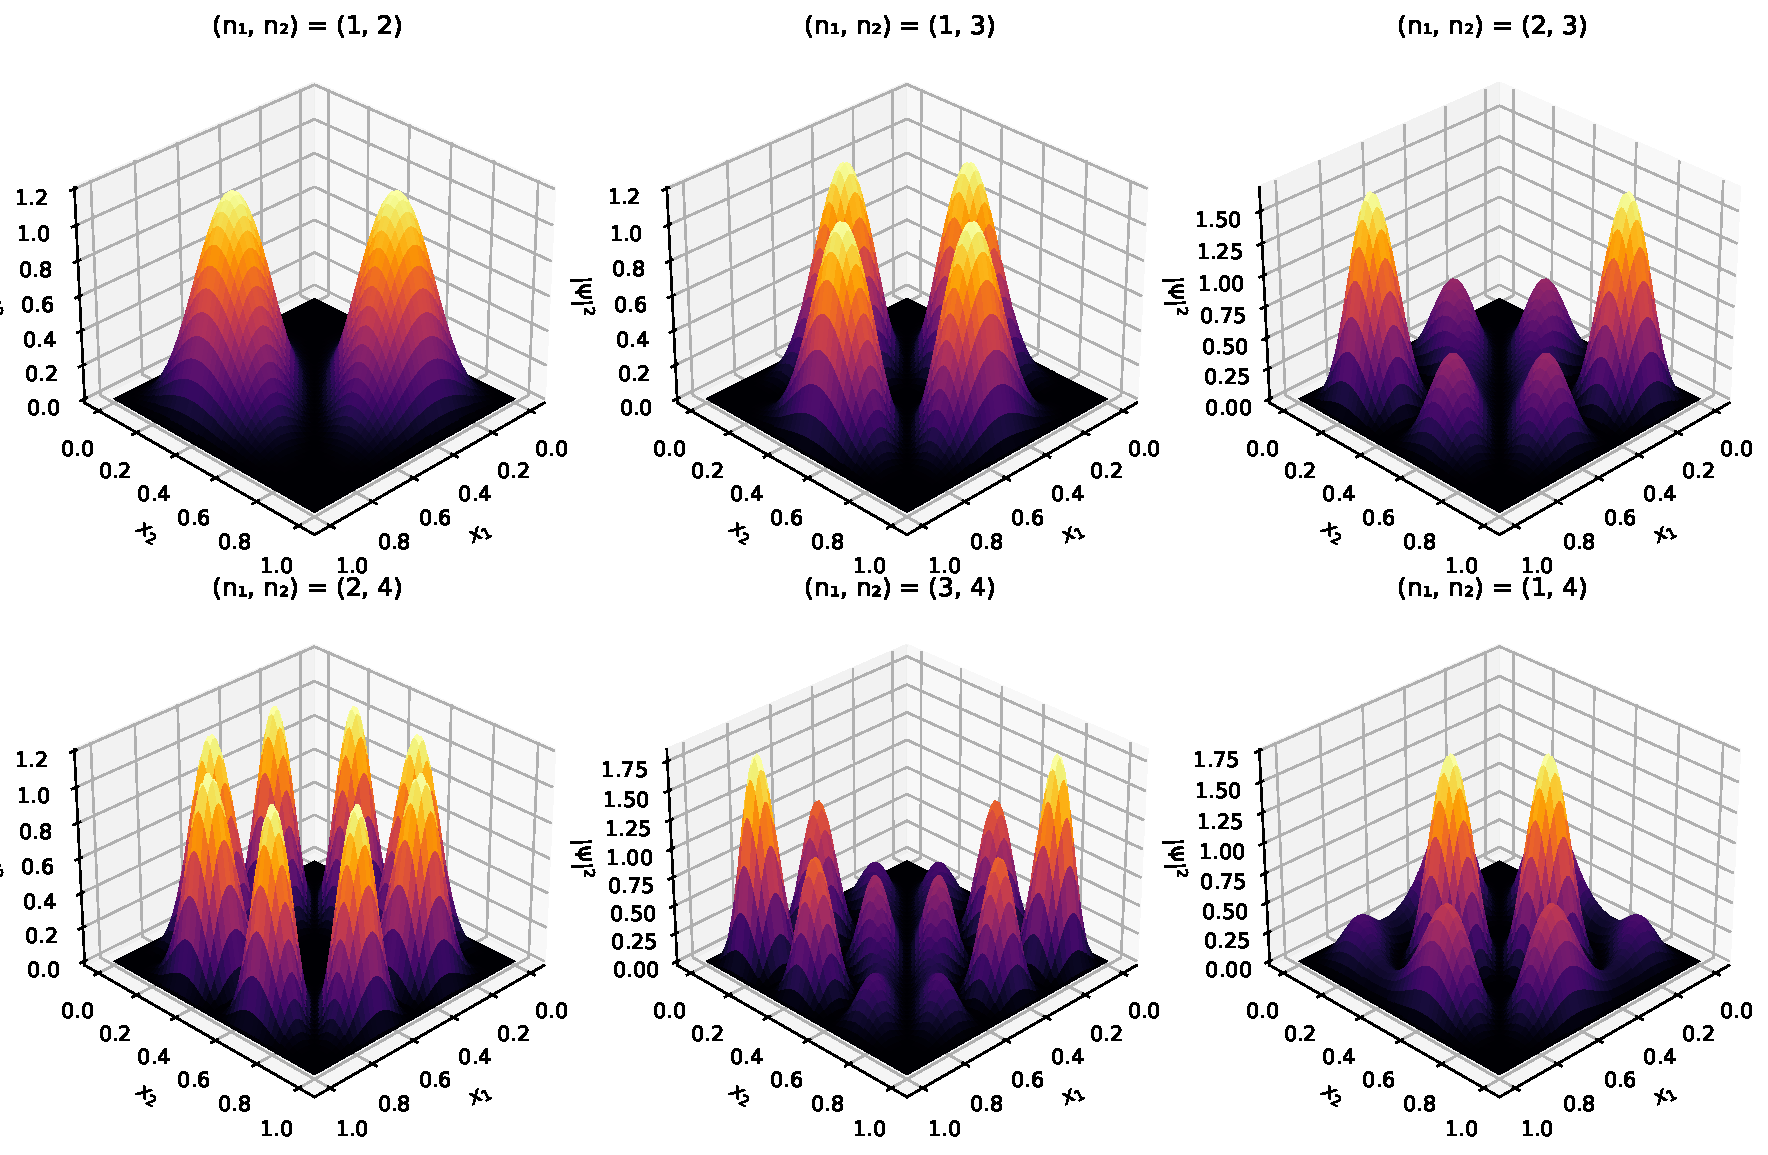
\includegraphics[width=0.9\textwidth]{./figures/fermions_3D_collage-1.pdf}
	\caption{Probability density $|\psi(x_1, x_2)|^2$ for six antisymmetric
		two-fermion configurations $\{n_1,n_2\} = \{1,2\}, \{1,3\}, \{2,3\},
	\{2,4\}, \{3,4\}, \{1,4\}$.}
	\label{fig:fermion_3D_collage}
\end{figure}

\Cref{fig:fermion_3D_collage} illustrates the spatial characteristics of
the fermionic states. Although the phase information is lost when
taking the modulus squared, a ``nodal line'' is clearly visible along
the diagonal $x_1 = x_2$, where the probability density is
identically zero.

As these are stationary states, the time evolution
$\Psi(x_1,x_2,t) = \psi(x_1,x_2)e^{-iEt/\hbar}$ introduces only a
global phase. The probability density is therefore static:
$|\Psi(x_1,x_2,t)|^2 = |\psi(x_1,x_2)|^2$.

It is crucial to contrast this result with the bosonic case.
The derivation above, which led to the vanishing of the interaction,
is valid only for the antisymmetric spatial sector (fermions).
For bosons, the spatial wavefunction $\psi_S(x_1, x_2)$ is symmetric,
so $\psi_S(x, x) \neq 0$. The delta interaction would therefore be
non-trivial, yielding corrections to the energy eigenvalues.

This fermionic solution trivially nullifies the delta contribution
only because we have assumed a spatially antisymmetric wavefunction.
This implies the fermions are either spinless (a theoretical construct)
or are in a spin-symmetric state (a triplet state),
which forces the spatial part to be antisymmetric.

If, however, the two fermions (e.g., electrons) were in a
spin-antisymmetric (singlet) state, the total wavefunction
$\ket{\Psi}_{\text{total}} = \ket{\psi}_{\text{spatial}}
\otimes \ket{\chi}_{\text{spin}}$
would require a spatially symmetric wavefunction $\psi_S(x_1, x_2)$
to maintain total antisymmetry. In that scenario,
$\psi_S(x, x) \neq 0$, the delta-function interaction would apply,
and the problem would become non-trivial.
